% Semantic Assistants - http://www.semanticsoftware.info/semantic-assistants
%
% This file is part of the Semantic Assistants architecture.
%
% Copyright (C) 2012, 2013 Semantic Software Lab, http://www.semanticsoftware.info
% The Semantic Assistants architecture is free software: you can
% redistribute and/or modify it under the terms of the GNU Affero General
% Public License as published by the Free Software Foundation, either
% version 3 of the License, or (at your option) any later version.
%   
% This program is distributed in the hope that it will be useful,
% but WITHOUT ANY WARRANTY; without even the implied warranty of
% MERCHANTABILITY or FITNESS FOR A PARTICULAR PURPOSE.  See the
% GNU Affero General Public License for more details.
% 
% You should have received a copy of the GNU Affero General Public License
% along with this program.  If not, see <http://www.gnu.org/licenses/>.

\chapter{Liferay Web Portal Integration}
\label{chap:liferay}
A web portal is a web-based software application, which provides a central entry point to a number of heterogeneous data sources. Portals are often used as enterprise information systems to enhance the communication and collaboration among users, such as Yahoo.com.\footnote{Yahoo!, \url{http://www.yahoo.com}} By means of personalized access to content, portal data can be adapted to its users and their assigned roles. A portal consists of several portlets, which are displayed as different data containers on the webpage. They are independent from each other, yet different communication techniques allow the transmission of information from one portlet to another.\footnote{For more information please refer to Java Specification Request (JSR 268), \url{http://jcp.org/en/jsr/detail?id=268}}

The \sa framework provides a custom portlet for Liferay\footnote{Liferay, \url{http://www.liferay.com}}, a popular open source portal, which allows its users to employ various text mining techniques on arbitrary portal content. For more information on the SA-Liferay integration please refer to our publication (\cite{LoefflerEtAl:CSWS2013}).

\section{Introduction}
As portals grow in size, one prominent issue that hinders their usability is associated with the wealth of information available in the portal repository. These mostly heterogeneous information are aggregated from various sources and presented to users based on their assigned roles. Ideally, an \emph{intelligent} portal must be able to offer content to users, taking into account contextual information beyond their roles and permissions. To this end, the portal needs to somewhat have an \emph{understanding} of what is available in the portal. Leveraging state-of-the-art techniques from the Natural Language Processing (NLP) domain allows portals to automatically process textual content. The SA-Liferay integration aims at bringing NLP power to this popular portal system and its users in a seamless, user-friendly manner.

\subsection{Use Cases of NLP in Portals}
In order to provide more concrete use cases of NLP techniques in the context of portals, we iterate over some example scenarios in the following.

\begin{description}
\item[Named Entity Recognition.] When dealing with large volume of textual documents or reading lengthy pages, a portal's \emph{intelligent assistants} can help users to automatically find named entities, such as persons, locations and organization names in a given text to quickly grasp an idea of the document at hand, without thoroughly reading the page. 
\item[Indexing Portal Content.] Ordinarily, an index page exists for large document collections that allows information seekers to find where in the collection a certain term is mentioned, much like the index found at the end of books. Using a combination of NLP techniques, one can automatically index the portal content and use it as a new facet for searching or discovering terms within the portal system.
\item[Automatic Summarization.] Another somewhat ambitious use case of NLP within the context of portals is the generation of automatic summarizes from one or a collection of selected documents. Automatically-generated focused or personalized summaries of portal content can help users find documents of interest in a more efficient way.
\end{description}

\noindent
%For some real-world examples on how the \wikinlp integration can be applied to
%various domains, please visit our
%\href{http://www.semanticsoftware.info/semantic-assistants-wiki-nlp-showcase}{showcase}
%web page.

\section{Installation}
The SA-Liferay integration consists of two components: a server-side component and a custom portlet to be installed on the portal. The server-side component is essentially an instance of the \sa server installed on a local or remote machine (see Chapter~\ref{chap:serv}). The \sa portlet available in our public repository is configured to connect to our public \sa server, but still can be modified to connect a custom endpoint (see Section~\ref{sec:server_change}). The \sa portlet has to be manually installed on the portal and configured to connect to the back-end \sa server in hold of a repository of various NLP pipelines, allowing users to invoke various services on the portal content. 

There are two options available to install the \sa portlet on a portal: You can merely deploy the portlet's binary file available in our public distribution\footnote{\sa Portlet WAR file, \url{http://assistant.cs.concordia.ca:8080/job/Semantic\%20Assistants\%20Liferay/lastSuccessfulBuild/artifact/liferay-plugins-sdk/dist/SemanticAssistants-portlet-6.1.1.1.war}} with its default configuration. Alternatively, if you would like to build the portlet binary file directly from the source code, or wish to modify the portlet's default behaviour (e.g., change the \sa server endpoint address), please refer to the Development Notes section at the end of this chapter.

Additionally, it is necessary to install the \sa theme (explained in Section~\ref{sec:theme_deploy}) and apply it to the webpage containing the \sa portlet for it to make use of the JavaScript library (jQuery) essential for inquiring and invoking the \sa portlet assistants. 

For activating the render parameters, which are necessary for the communication among the portlets, please add the following line to your \texttt{portal-ext.properties} file: 

%\centering
\begin{lstlisting}[language=XML,numbers=left,xleftmargin=4mm,columns=flexible]
portlet.public.render.parameter.distribution=ALL_PORTLETS
\end{lstlisting}

Note that the following instructions are based on a Liferay Portal server installation version 6.1.1 CE GA2. 

\subsection{\sa Portlet Deployment}
In order to deploy the \sa portlet into your portal, you have to copy the \texttt{SemanticAssistantsPortlet.war} file into the \texttt{deploy} folder of your Liferay installation. Liferay polls on this folder every few seconds, so it will find the new portlet and deploy it automatically. As soon as the deployment is successful, the new portlet will be available in the general portlet container and similar to other portlets in Liferay, the \sa portlet can be added to any portal web page. In order to add the \sa portlet, choose \texttt{Add \textgreater~More} from the top menu and then you can find the portlet under the \sa category and click on the \texttt{add} link or drag the portlet name into the desired web page as shown in Figure~\ref{fig:liferay_add_portlet}.

\begin{figure}
\centering
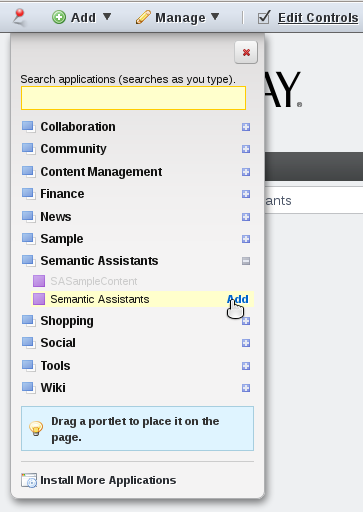
\includegraphics[scale=0.6]{pictures/liferay_add_portlet.png}
\caption{Adding the \sa Portlet to a Page}
\label{fig:liferay_add_portlet}
\end{figure}

\subsection{Theme Deployment}
\label{sec:theme_deploy}
Several functions in the \sa portlet need the jQuery library for a successful execution. Thus, you have to download and install the \sa theme available in our build server. Simply copy the \texttt{SemanticAssistantTheme.war} file from our public distribution into the deploy folder of your Liferay installation. Liferay automatically detects and deploys the new component. Then go to your Liferay portal, login in and browse to the webpage that contains the \sa portlet. From the top of the page select \texttt{Manage \textgreater~Page}. From the right-hand sidebar select ``Look and Feel'' to switch the theme associated with the \sa portlet. From the presented dialog, under the ``Define a specific look and feel'', select the \sa theme for your portlet.

\section{User Interface}
Once the portlet is added to the page, you can inquire about available NLP services by selecting a \sa endpoint from the provided combobox. Selecting a server address will dynamically load the list of available services along with their description and runtime parameters. To select an assistant, click on the service's name in order to expand the service information box as shown in Figure~\ref{fig:liferay_sa_portlet}. Optionally, you can customize the execution of the NLP pipelines by modifying their runtime parameters.

\begin{figure}
\centering
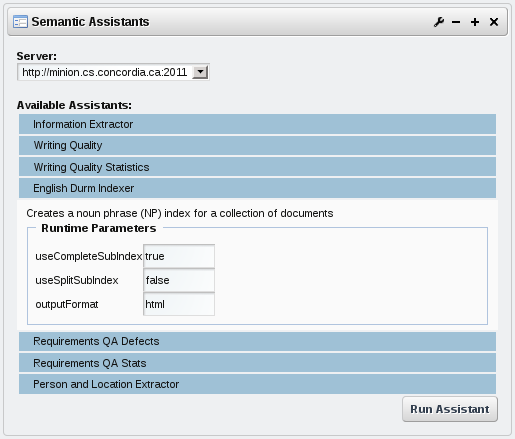
\includegraphics[scale=0.7]{pictures/liferay_sa_portlet.png}
\caption{\sa Portlet User Interface in Liferay}
\label{fig:liferay_sa_portlet}
\end{figure}

\blankline

In order to invoke an assistant, you need to first provide the content that is going to be analyzed. Therefore, other portlets in the page must provide a mechanism to initialize specific global variables\footnote{Also known as public rendering parameters in Liferay terminology} that the \sa portlet is listening to. As an example, the \sa integration for Liferay also includes a sample portlet containing an example text for demo purposes. The \emph{SASampleContent} can be found in the \texttt{Clients/Portal/Liferay/SASampleConent} and deployed similar to the \sa portlet. When deployed, the SASampleContent portlet provides two buttons, one intended for sending the portlet text to the \sa portlet for analysis and the other for clearing the results from the sample portlet's original content. Figure~\ref{fig:liferay_both_portlets} shows both the aforementioned portlets in a page.

\begin{figure}
\centering
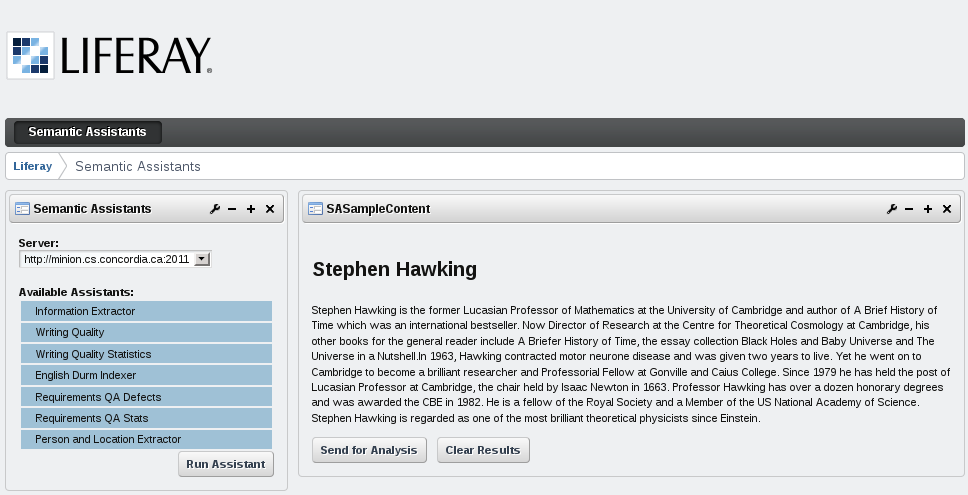
\includegraphics[scale=0.6]{pictures/liferay_both_portlets.png}
\caption{\sa portlet together with a sample content portlet}
\label{fig:liferay_both_portlets}
\end{figure}

You can send the content portlet text for analysis by clicking on the ``Send for Analysis'' button. Then choose a server endpoint address from the \sa portlet combobox and select a desired service to be executed on the provided content. In Figure~\ref{fig:liferay_results_portlet}, you can see the ``Person and Location Extractor'' service results ran on the provided content. The offsets of the NLP results are used to highlight the terms in the portlet's original content.

\begin{figure}
\centering
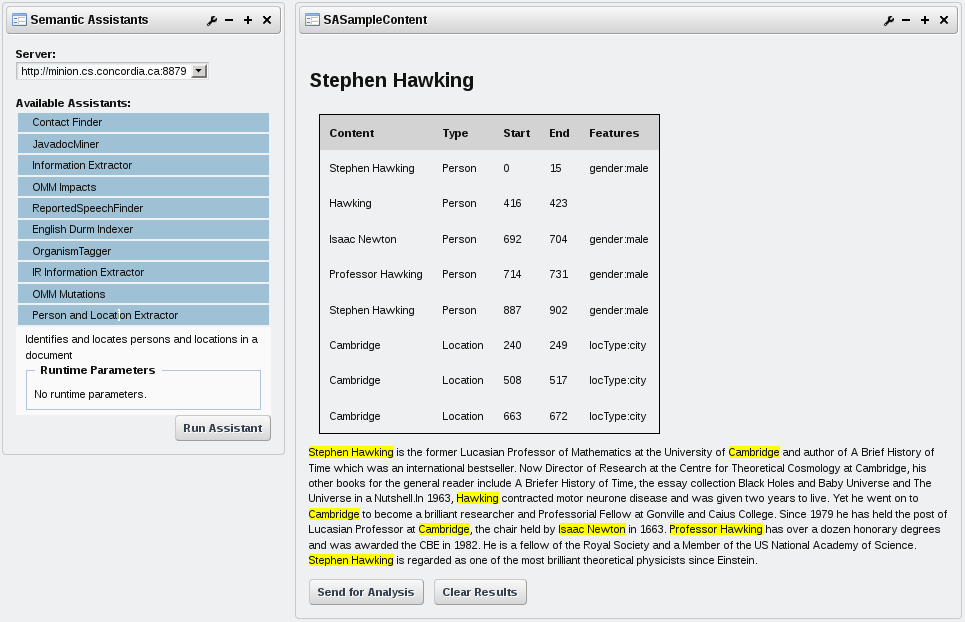
\includegraphics[scale=0.6]{pictures/liferay_results_portlet.png}
\caption{NLP Results highlighted in a sample content portlet}
\label{fig:liferay_results_portlet}
\end{figure}

\section{Development Notes}
In this section, we provide further details on the underlying architecture of the \sa-Liferay integration and explain how you can modify the default behaviour of the \sa portlet.

\subsection{System Architecture}
Our novel \sa-Liferay integration architecture, illustrated in Figure~\ref{fig:liferay_arch}, is designed to allow various portlets to benefit from NLP techniques on their content. The core idea is to enable generic portlets to communicate with the \sa portlet, specifically designed to connect to the back-end \sa server and provide inquiry and invoking capability of NLP pipelines to portal users. 

\begin{figure}[h]
\centering
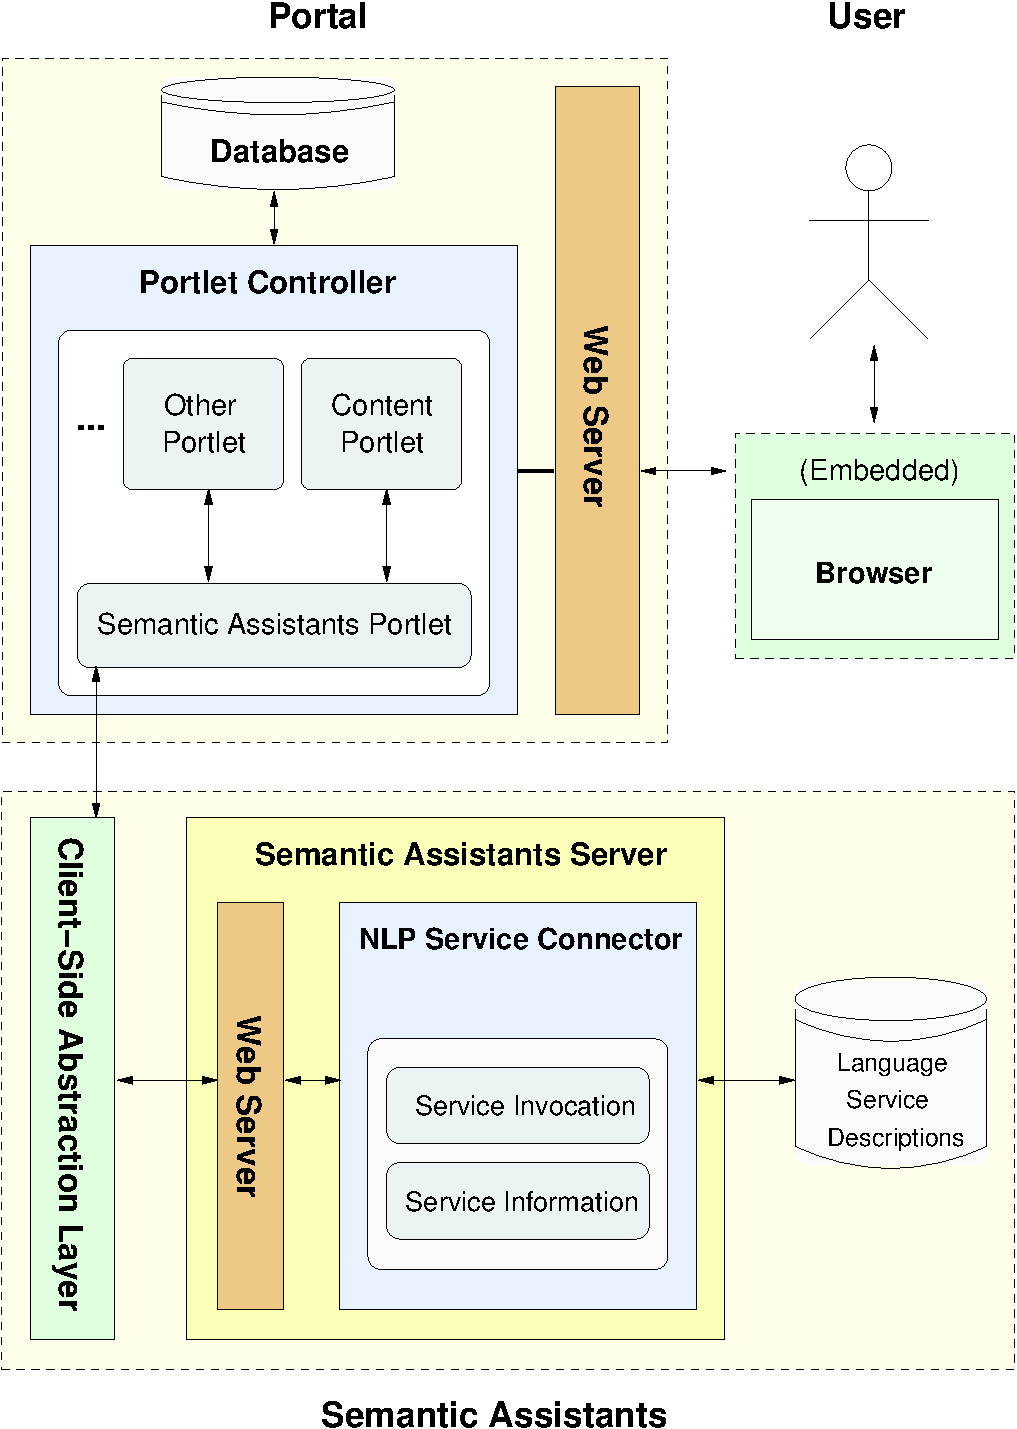
\includegraphics[scale=0.33]{pictures/liferay_arch.pdf}
\caption{The \sa-Liferay integration architecture}
\label{fig:liferay_arch}
\end{figure}

In this architecture, all available portlets in a page can communicate with the \sa portlet by sending content for analysis and receiving the results. To commence an analysis session, users interact with the portal via their web browser, for example, on their desktop computer or from a mobile device. Through this integration, users can select an NLP service to execute on a portlet's content from a dynamically-generated list of available \emph{assistants} in the \sa server repository. An execution request is then sent to the \sa server from the \sa portlet in form of a W3C\footnote{World Wide Web Consortium (W3C), \url{http://www.w3.org}} standard web service call that triggers the execution of the designated NLP pipeline on the provided content. The results of each successful service execution are first received by the \sa portlet and then passed on to the portlet that requested the service execution. The NLP pipelines are described in the OWL\footnote{Web Ontology Language, \url{http://www.w3.org/2004/OWL/}} language and the \sa server uses SPARQL\footnote{SPARQL Query Language, \url{http://www.w3.org/TR/rdf-sparql-query/}} for a dynamic discovery of available services upon each user request (see Chapter~\ref{chap:dev}). Hence, adding or removing NLP services to the integration requires no modification to the code base of the portal. In addition, the default behaviour of passing the NLP results to the portlet containing the source content can be configured by the portal developers, so that any other portlet can receive the results by reading them from a global variable. This feature allows for a multitude of different applications of NLP services in the context of web portals.

\subsection{Project Directory Structure}
The directory structure of the \sa portlet found in \texttt{Clients/Portal/Liferay/} is as follows:

\begin{description}
\item [build.xml] This is a custom ANT script for automatically resolving the portlet's dependencies.
\item [docroot] Main resource folder of the portlet.
\begin{description}
\item[css] Contains Cascading Style Sheet documents for the portlet user interface.
\item[js] Contains JavaScript files for the portlet's service inquiry and invocation.
\item[jsp] Contains the front-end interface of the portlet.
\item[META-INF] Contains metadata of the portlet -- used during packaging of the portlet into a binary archive file.
\item[WEB-INF] Contains the actual source code of the portal, as well as referenced libraries and configuration files.
\end{description}

\item [ivy.xml] Enlists the dependencies of the portlet source code. Whatever dependencies are listed in this XML file will be searched for and downloaded by Ivy.
\item [ivysettings.xml] Describes the Ivy configuration, such as the list of software repositories.
\end{description}

\subsection{Deploying Portlets from Source Code}
\label{sec:src_deploy}
As mentioned earlier in this chapter, the \sa portal can also be deployed to a Liferay portal by building it directly from the source code. To do so, you will need to download the Liferay SDK\footnote{Liferay Plugins SDK,~\url{http://www.liferay.com/community/wiki/-/wiki/Main/Plugins+SDK}} and have ANT installed in your system. Follow the provided steps below:

\begin{enumerate}
\item Copy the \texttt{SemanticAssistants-portlet} folder in the \texttt{portlets} folder of your Liferay SDK.
\item Browse to the \sa portlet top-level directory (which contains the \texttt{build.xml} file) in your terminal and type ``\texttt{ant resolve}''. This will automatically download all the project's dependencies so you can compile and build the portlet's WAR file.
\item Upon a successful execution of step 2, type ``\texttt{ant deploy}''. This will create the portlet's WAR file and copy it to your Liferay SDK \texttt{dist} folder.
\item You can now copy the generated WAR file to the \texttt{deploy} folder of your Liferay installation.
\end{enumerate}

\subsection{Inter-Portlet Communication}
Portlets are able to communicate among each other. The JSR 268 standard\footnote{JSR 268 Standard, \url{http://www.jcp.org/en/jsr/detail?id=268?}} describes different techniques for a successful transmission of information from one portlet to another. In our project we have concentrated on the communication based on render parameters, which are defined in the \texttt{portlet.xml} file within the SemanticAssistants-portlet \texttt{/docroot/WEB-INF} folder. In order to change or to add parameters, please open the \texttt{portlet.xml} file and scroll down to the public-render-parameter section. As you can see, we have defined the public render parameters \texttt{sa\_text}, \texttt{sa\_result} and \texttt{sa\_result\_type}. \texttt{sa\_text} contains the text which is going to be transmitted to the \sa, \texttt{sa\_result} comprises the whole result coming back from the SA server and the \texttt{sa\_result\_type} defines the result type, described later in the following subsection. After this registration those parameters are available for all other portlets. The receiver portlet only needs to define the same parameters in the same way in its own \texttt{portlet.xml}. Within the code you have access to the parameters with: \url{request.getParameter(``sa\_text'');} or you can set the parameters with the method \url{response.setRenderParameter(``sa\_text'', ``someText'');}.

Please make sure, that you have set the following line in our portal-ext.properties file to activate the inter-portlet communication:

\begin{lstlisting}[language=XML,numbers=left,xleftmargin=4mm,columns=flexible]
portlet.public.render.parameter.distribution=ALL_PORTLETS
\end{lstlisting}

For a further detailed description about using render parameters in Liferay, please visit the Liferay wiki\footnote{Liferay Wiki, \url{https://www.liferay.com/de/community/wiki/-/wiki/Main/Portlet+to+Portlet+Communication}}. 

\subsection{Embedding NLP Results in Your Own Portlet}
Depending on the NLP service chosen by users, there are three types of service results  (see Section~\ref{sec:response}) that can be generated by the \sa server and returned to the portlet.

\begin{itemize}
\item When an NLP pipeline generates ``Annotation'' type results, the \sa portlet represents the list of annotations as an array of JSON objects. An example JSON array representing two annotation instances of different types is shown in Figure~\ref{list:json_annot}.
\begin{figure}[h!]
\centering
\begin{lstlisting}[language=Java,numbers=left,xleftmargin=4mm,columns=flexible]
[
   [
      {"mType":"Person","mContent":"Stephen Hawking","mFeatures":{"gender":"male"},"mStart":0,"mEnd":15},
   ],
   [
      {"mType":"Location","mContent":"Cambridge","mFeatures":{"locType":"city"},"mStart":240,"mEnd":249},
   ]
]
\end{lstlisting}
\caption{Example JSON array of \texttt{ANNOTATION} result type}
\label{list:json_annot}
\end{figure}

\item When the result of an NLP service execution is a ``Boundless Annotation''. the \sa portlet generates a list of JSON objects representing the boundless annotations. The length of the JSON array is always 1. A sample result of this type is similar to Figure~\ref{list:json_annot}, except that it always has the description of exactly one object in it.
\item When the result of an NLP service execution is a ``File'', the \sa portlet will return the content of the file as a string along with the file's MIME type.
\end{itemize}

\subsection{Modifying the \sa Server Endpoint}
If you would like to modify the \sa server addresses in the portlet combo box, you have to modify the \texttt{view.jsp} file found in the project's \texttt{jsp} folder. The server endpoint addresses are kept in an array list, therefore, an arbitrary number of entries can be added to or removed from the list. Find the following lines in the JSP file and modify it to your needs.

\begin{figure}[h!]
\centering
\begin{lstlisting}[language=Java,numbers=left,xleftmargin=4mm,columns=flexible]
List<String> servers = new ArrayList<String>();
servers.add("http://minion.cs.concordia.ca:8879");
servers.add("http://www.example.com:1234");
\end{lstlisting}
\caption{List of \sa server endpoints in the portlet}
\label{list:portal_server_addresses}
\end{figure}

Note that after applying your modifications, you will need to recompile the portlet and build a new WAR file to be re-deployed on the portal.

\label{sec:server_change}